\documentclass{beamer}
\usetheme{Montpellier}
\usecolortheme{seahorse}

\usepackage[slovak]{babel}
\usepackage[utf8x]{inputenc}

\usepackage{pdfpcnotes}

\newcommand{\bigO}{\ensuremath{\mathcal{O}}}

\title{Cache-oblivious algoritmy a ich vizualizácia}
\author[Ladislav Pápay]{Ladislav Pápay \\ ~ \\ Vedúci: Mgr. Jakub Kováč, PhD.}
\date{16.04.2014}

\begin{document}

\frame{\titlepage}

\section{Úvod}
\begin{frame}
    \frametitle{Ciele práce}
    \begin{itemize}
        \item Vysvetlenie pamäťového modelu
        \item Prehľad cache-oblivious algoritmov a DŠ
        \item Vizualizácia vybraných DŠ
    \end{itemize}
\end{frame}

\section{Pamäťový model}
\subsection{External-memory model}
\begin{frame}
    \frametitle{External-memory model}
	\begin{columns}[T]
		\begin{column}{.4\textwidth}
			\begin{itemize}
				\item Cache celkovej veľkosti $M$
				\item Obsahuje $N = \frac{M}{B}$ blokov veľkosti $B$
				\item Disk (neobmedzenej) veľkosti
				\item Počíta sa počet prenesených blokov (operácie v cache sú zadarmo)
			\end{itemize}
		\end{column}
		\begin{column}{.6\textwidth}\raggedleft
			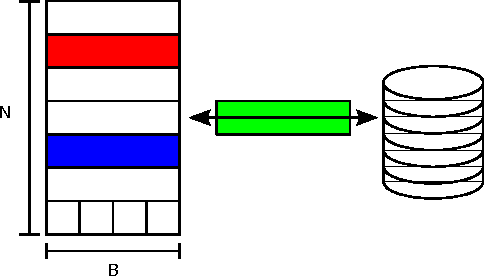
\includegraphics[scale=0.75]{../figures/external_memory_inkscape/drawing.pdf} 
		\end{column}
	\end{columns}
	%\input{../figures/external_memory_inkscape/drawing.eps_tex} 
\end{frame}

\begin{frame}
	\frametitle{External-memory model}
	\begin{itemize}
		\item Známe tiež ako cache-aware (kontrast voči cache-oblivious)
		\item Poznáme $B$ a $M$, každá operácia čítania/zápisu na disk je explicitne vykonaná algoritmom
		\item Ak je cache plná musí vybrať, ktorý blok zahodí
	\end{itemize}
	\pnote{Pri zahadzovani bloku v cache ak bol zmeneny treba zapisat}
\end{frame}

\begin{frame}
	\frametitle{Problémy}
	\begin{itemize}
		\item Treba explicitne čítať a zapisovať bloky, riešiť asociatívnosť cache
		\item Čo ak sa zmenia parametre $B$ alebo $M$?
		\item Čo v prípade viac úrovní? Treba pre každú susediacu dvojicu poznať $B, M$  a spravovať bloky
	\end{itemize}
	\pause
	\begin{center}
		\begin{tabular}{|l|l|l|}
			\hline
			Úroveň & Veľkosť & Odozva \\ \hline
			L1 & $\approx$ 128KiB & 4clk $\approx$ 1ns (pri 3.5GHz) \\ \hline
			L2 & $\approx$ 1MiB & 10-12clk $\approx$ 3ns (pri 3.5GHz) \\ \hline
			L3 & $\approx$ 8MiB & 20-50clk $\approx$ 10ns (pri 3.5GHz) \\ \hline
			RAM & $\approx$ 4GiB & $\approx$ 100ns \\ \hline
			Disk & $\approx$ 1TiB & $\approx$ 0.1-10ms \\
			\hline
		\end{tabular}
	\end{center}
	\pnote{B pre disk/ram je cca 4KB}
	\pnote{Zistenie B a M - pri kompilacii, za behu?}
	\pnote{Treba pri zmene prekompilovat? Prepisat algoritmus}
	\pnote{L3 - RAM : 10x pomalsie, 100x vacsie}
	\pnote{RAM - Disk: 1 000x - 100 000x pomalsie, 1000x vacsie}
\end{frame}

\subsection{Cache-oblivious model}
\begin{frame}
	\frametitle{Cache-oblivious model}
	\begin{itemize}
		\item Rovnaká architektúra, presun blokov prebieha automaticky
		\begin{itemize}
			\item Predpokladá optimálne nahrádzanie blokov (offline), ale FIFO/LRU je len konštantne horšie
		\end{itemize}
		\item Chceme (asymptoticky) rovnaký počet presunov ako optimálny cache-aware algoritmus, ale bez znalosti parametrov $B$ a $M$
	\end{itemize}
	\pnote{Pozname pri analyze, ale nie pocas behu}
\end{frame}

\section{Algoritmy a dátové štruktúry}
\subsection{Statický strom}
\begin{frame}
    \frametitle{Statický strom}
    \begin{itemize}
        \item Binárny vyhľadávací strom
        \item V pamäti uložený podľa {\em van Emde Boas} usporiadania
        \begin{itemize}
            \item Rozdelíme uprostred na horný podstrom a $\sqrt{N}$ spodných podstromov veľkosti $\sqrt{N}$
            \item Tie rekurzívne rozdelíme a uložíme do súvislého bloku pamäte
        \end{itemize}
    \end{itemize}
    \begin{center}
        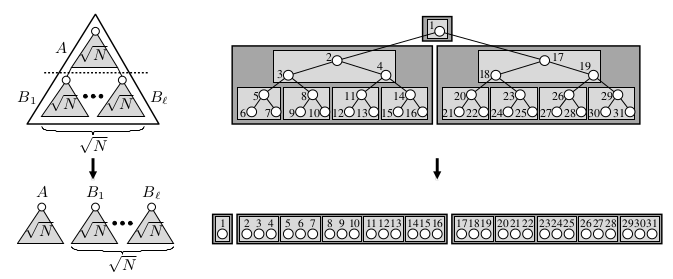
\includegraphics[width=0.8\textwidth,]{../figures/downloaded_dont_use/cobplus-tree-crop.png}
    \end{center}
\end{frame}

\begin{frame}
    \frametitle{Analýza}
    \begin{itemize}
        \item Vyhľadávanie ako v klasickom BST (cache-ignorant prístup)
        \begin{itemize}
            \item Pozrime sa na takú úroveň delenia, že sú podstromy $\le B$ a teda zmestia sa do najviac dvoch blokov
            \item Tieto podstromy majú výšku $< \lg{B}$ ale $\ge \frac{1}{2}\lg{B}$
            \item Vyhladávanie prejde cestu od koreňa do listu dĺžky $\lg N$
            \item Prejdeme najviac cez $\frac{\lg N}{\frac{1}{2}\lg{B}}$ podstromov a na každý treba najviac 2 pamäťové presuny
        \end{itemize}
        \item Spolu teda $\bigO(\log_{B}{N})$ čo je spodná hranica pre external-memory model
    \end{itemize}
    \pnote{Analogia v cache-aware je B-strom}
\end{frame}

\subsection{Ordered file}
\begin{frame}
    \frametitle{Ordered file}
    \begin{itemize}
        \item Problém: udržiavať usporiadanú postupnosť prvkov, možnosť vkladať/odstraňovať, ako pole veľkosti $\bigO(N)$ $\Rightarrow$ medzery $O(1)$, vieme rýchlo prechádzať
        \item Riešenie: rozdelíme súvislé pole na imaginárne bloky veľkosti $\bigO(\log N)$ a vyrobíme nad nimi imaginárny úplný binárny strom
        \item {\em Hustota} vrcholu bude $\frac{\text{počet plných}}{\text{kapacita}}$, udržiavame podla istých hraníc aby nebolo príliš plné (nie je kam vložiť) ani príliš prázdne (pomalé prechádzanie)
    \end{itemize}
    \pnote{Hranice hustoty:}
    \pnote{Listy: 1/4 - 1}
    \pnote{Koren: 1/2 - 3/4}
\end{frame}

\begin{frame}
\begin{center}
        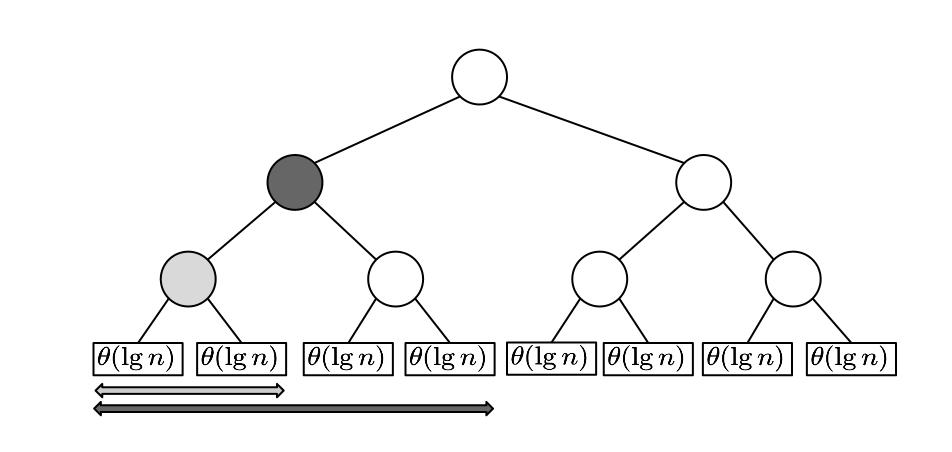
\includegraphics[width=0.8\textwidth,]{../figures/downloaded_dont_use/fig2-ofm.jpg}
    \end{center}
\end{frame}

\begin{frame}
    \frametitle{Operácie}
    \begin{itemize}
        \item {\em Vloženie prvku}: Upravíme blok a postupujeme hore v strome, kým nenájdeme vrchol, ktorý má hustotu v medziach a rovnomerne prerozdelíme prvky v príslušných blokoch
        \item {\em Zmazanie prvku} podobne
        \item Každá operácia upraví súvislý interval veľkosti $\bigO(\lg^2 N)$
    \end{itemize}
    \pnote{Imaginarny strom, scan v dvoch smeroch}
    \pnote{Odhad - amortizovane, dá sa aj worst-case}
    \pnote{Conjencture lowerbound}    
\end{frame}

\subsection{Dynamický strom}
\begin{frame}
    \frametitle{Dynamický strom}
    \begin{itemize}
        \item Skombinujeme predošlé dve štruktúry a dostaneme dynamický vyhľadávací strom
        \item Máme OF v ktorom sú kľúče a medzery, použijeme ako listy pre BST uložený v vEB layoute
        \item Vo vnútorných uzloch ukladáme maximum z podstromov
    \end{itemize}
    \begin{center}
        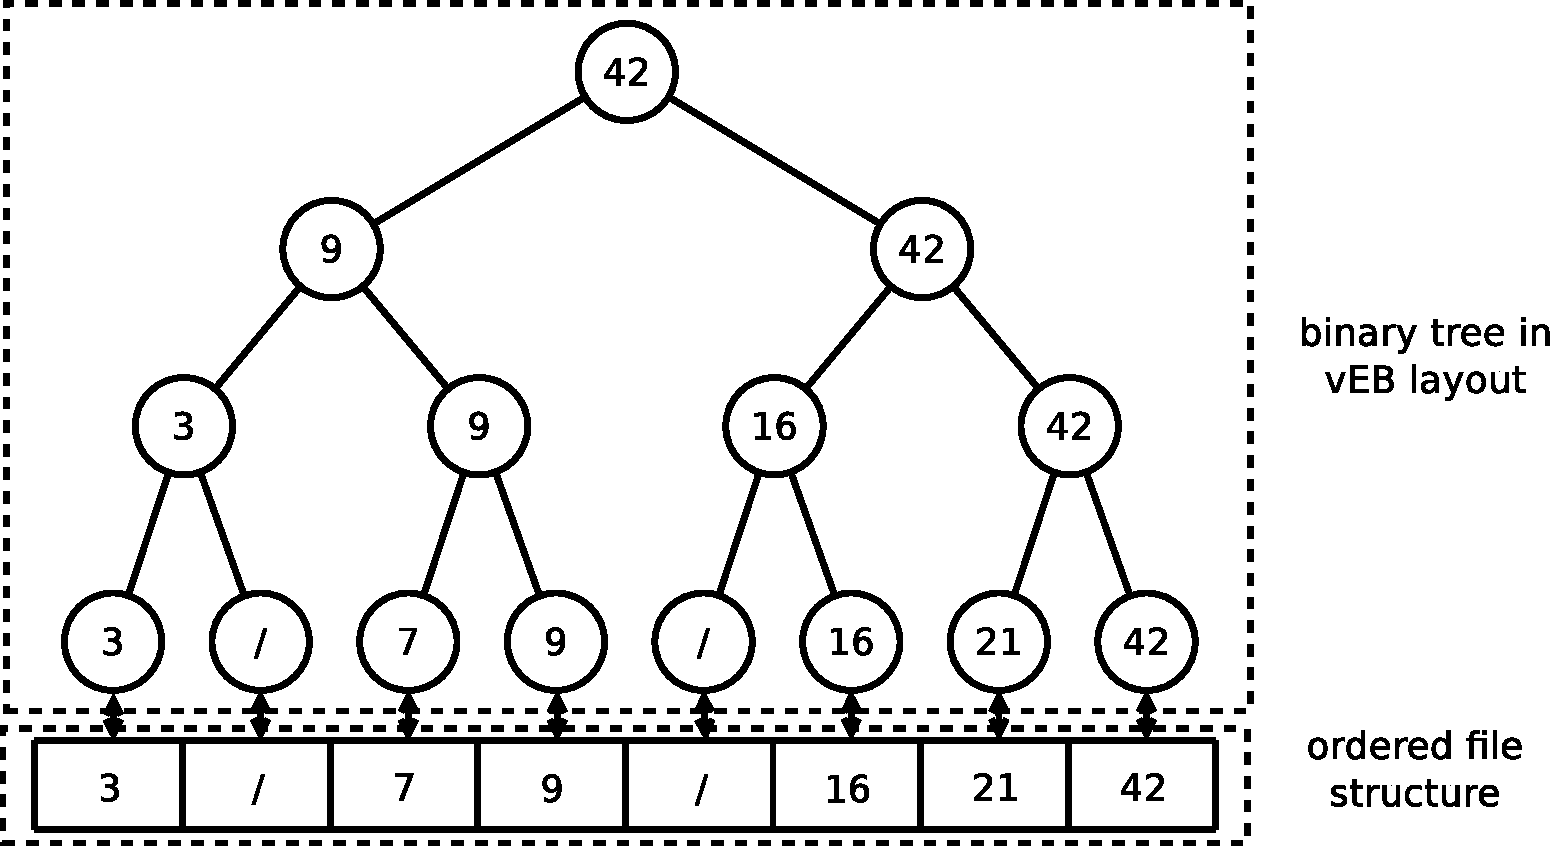
\includegraphics[height=0.5\textheight]{../figures/downloaded_dont_use/vEBpOFM.pdf}
    \end{center}
\end{frame}

\begin{frame}
    \begin{itemize}
        \item Vyhľadávanie: rovnako ako v statickom $\bigO(\log_B N)$
        \item Vkladanie
        \begin{itemize}
            \item Nájdeme nasledujúci kľúč v OF, vložíme nový pred neho
            \item Musíme upraviť strom pre zmenený interval veľkosti $\bigO(\lg^2 N)$
            \item Prechod cez zasiahnuté vnútorné uzly vyžaduje $\bigO(\frac{\lg^2 N}{B})$ pamäťových operácií
        \end{itemize}
        \item Vkladanie a odstraňovanie spolu potrebuje $\bigO(\log_B N + \frac{\lg^2 N}{B})$
        \item Dá sa zredukovať na $\bigO(\log_B N)$ ak ukladáme $\bigO(\log N)$ bloky
    \end{itemize}
    \begin{center}
        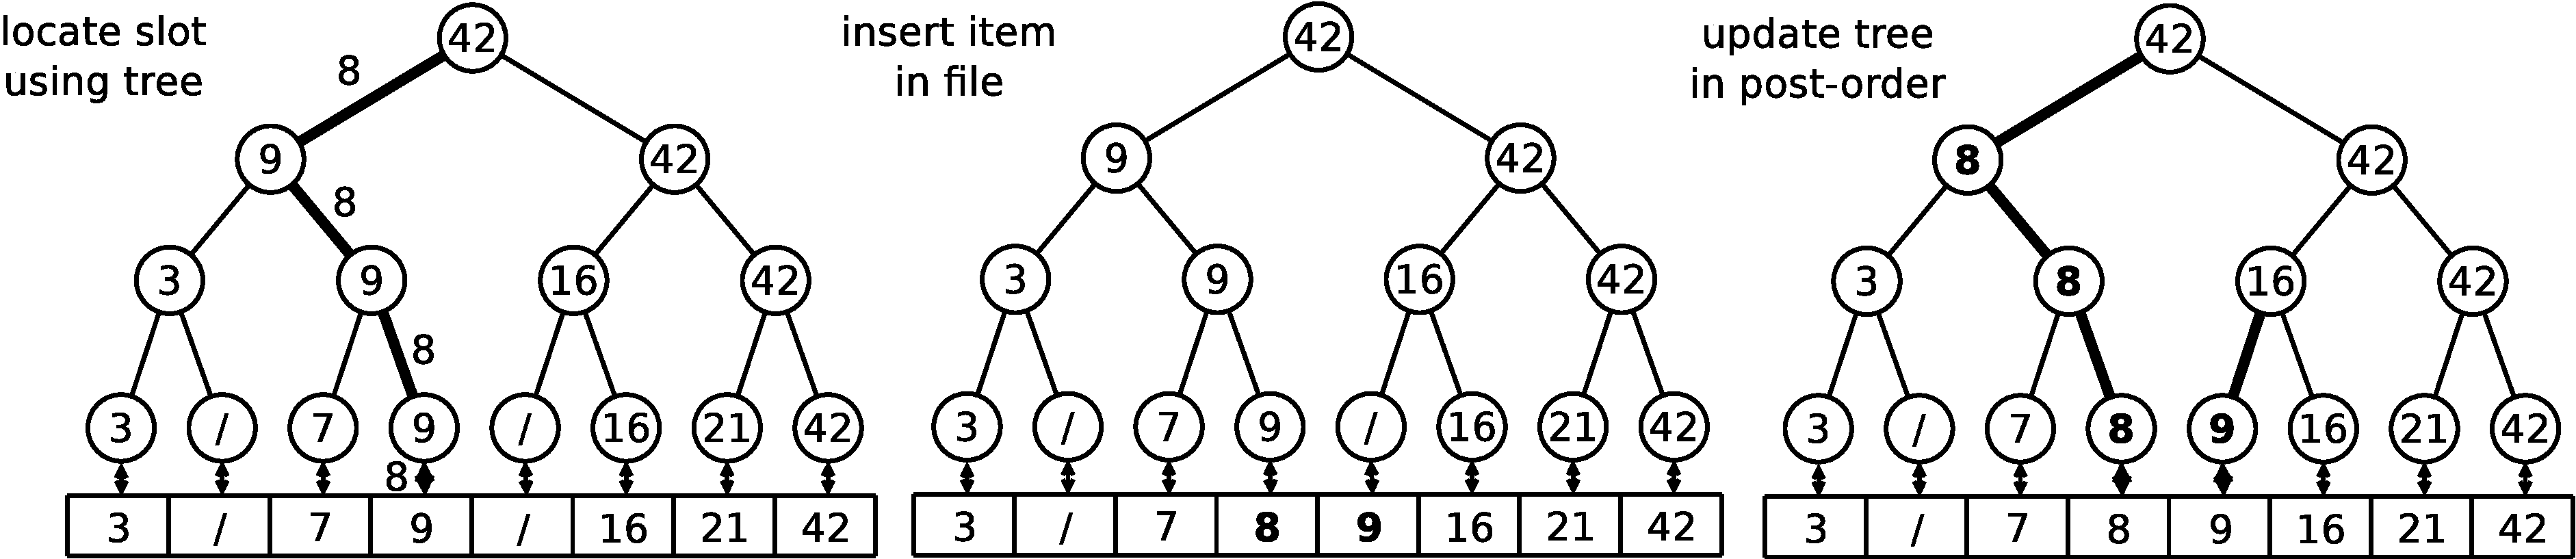
\includegraphics[width=\textwidth]{../figures/downloaded_dont_use/dyn-insert.pdf}
    \end{center}
\end{frame}

\section{Vizualizácie}
\begin{frame}
    \frametitle{Vizualizácie}
    \begin{itemize}
        \item Pridanie týchto troch DŠ do {\em alg-vis} (+ možno ďalšie)
        \item Krokovanie s animáciami, vysvetlenie krokov, undo/redo, \dots
    \end{itemize}
    \begin{center}
        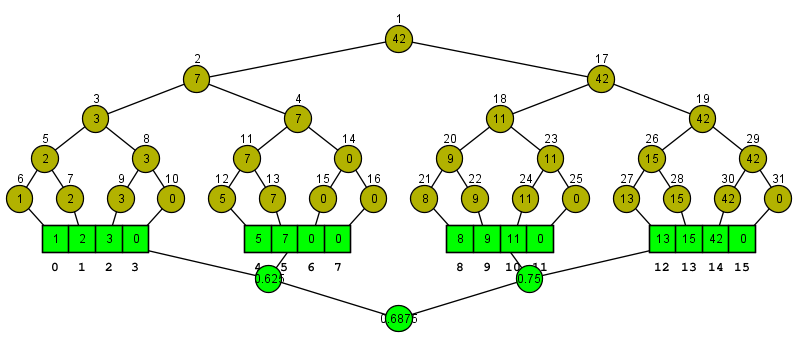
\includegraphics[width=\textwidth]{../figures/screenshots/slides_cobtree.png}
    \end{center}
\end{frame}

\end{document}